%==============================================
\begin{algorithm}[t!]
\caption{Physics-Informed Hybrid Search}\label{alg:push}
\SetAlgoLined
\KwIn{$\mathbf{s}_0$, $\alpha$, $\mathsf{EvalSim}(\cdot)$, $W$--criterion by~\eqref{eq:wccg_criterion}}

\KwOut{$\pi^\star$}
\tcc{Initialization}
$\nu_0\gets(\mathbf{s}_0,\emptyset),\;\chi(\nu_0)=0$\;
Init $\mathcal{Q}$ by~\eqref{eq:priority}\;
\While{not terminated}{
  \tcc{Selection}
  $\nu\gets\mathcal{Q}.\texttt{pop\_min}()$ by~\eqref{eq:priority}\;
  \tcc{Parallel Expansion}
  \ForEach{$g\in\mathsf{Rank}(\nu)$}{
    \ForEach{$(\mathbf{v},\boldsymbol{\xi})\in\Xi_g$}{
    $\tau=(g,\mathbf{v},\boldsymbol{\xi})$\;
    $(\mathbf{s}',\delta_T,\delta_J)\gets\mathsf{EvalSim}(\nu,\tau)$ by~\eqref{eq:sim}\;
    \If{success}{
      $\nu'\gets(\mathbf{s}',\pi\cup\{\tau\})$\;
      $\chi(\nu')\gets\chi(\nu)+\delta_\texttt{T}+\alpha\,\delta_\texttt{J}$\;
      $\mathcal{Q}.\texttt{push}(\nu')$\;
      }
    }
  }
  \tcc{Termination Check}
  \If{$\mathbf{s}'$ admits $\mathcal{P}^W_{\texttt{V}}$ by~\eqref{eq:wccg_criterion}}{
    $\pi^\star\gets\pi'$, \textbf{break}\;
  }
}
\Return $\pi^\star$;
\end{algorithm}
%==============================================



%==============================================
\subsection{Physics-Informed Hybrid Search}\label{subsec:simloop}

The hybrid search couples high-level decisions about blocking gaps with
low-level feasibility of multi-robot pushing. Unlike purely geometric
planners, this procedure simultaneously determines a sequence of gaps to clear
and physically feasible pushing actions, including directions, contact modes,
and forces. Parallel physics simulation is embedded so that many candidate
push strategies can be evaluated simultaneously at each expansion, and the resulting
successor states are returned to the search. This tight coupling of discrete
graph reasoning with continuous pushing dynamics is unique for the considered problem.

\subsubsection{Tree and Initialization}
The search tree $\mathcal{T}$ is composed of nodes
$\nu\triangleq(\mathbf{s},\pi)$, where $\mathbf{s}$ is the current system
state including the positions and orientations of all robots and movable
obstacles as in~\eqref{eq:transition}, and $\pi$ is the partial pushing
strategy realized so far as in~\eqref{eq:schedule}. Two global functions are
maintained: $\mathsf{Rank}(\nu)$ stores a ranked list of candidate gaps at this
node together with their exploration status, derived from~\eqref{eq:pred_cost};
and $\chi(\nu)$ returns the cumulative execution cost
from the root to $\nu$.
The root is initialized as
$\nu_0\triangleq(\mathbf{s}_0,\emptyset)$, where
$\mathbf{S}^{\texttt{S}}$ corresponds to the initial system state
$\mathbf{s}_0$. At initialization, $\chi(\nu_0)=0$, and
$\mathsf{Rank}(\nu_0)$ is constructed by first computing the frontier loop
$\mathcal{L}_\nu$ associated with~$\mathbf{s}_0$, then extracting the visible
gaps $\Gamma_{\mathcal{L}_\nu}$, and finally ranking them by their predicted
cost-to-connect.
%------------------------------
\begin{figure}[t!]
  \centering
  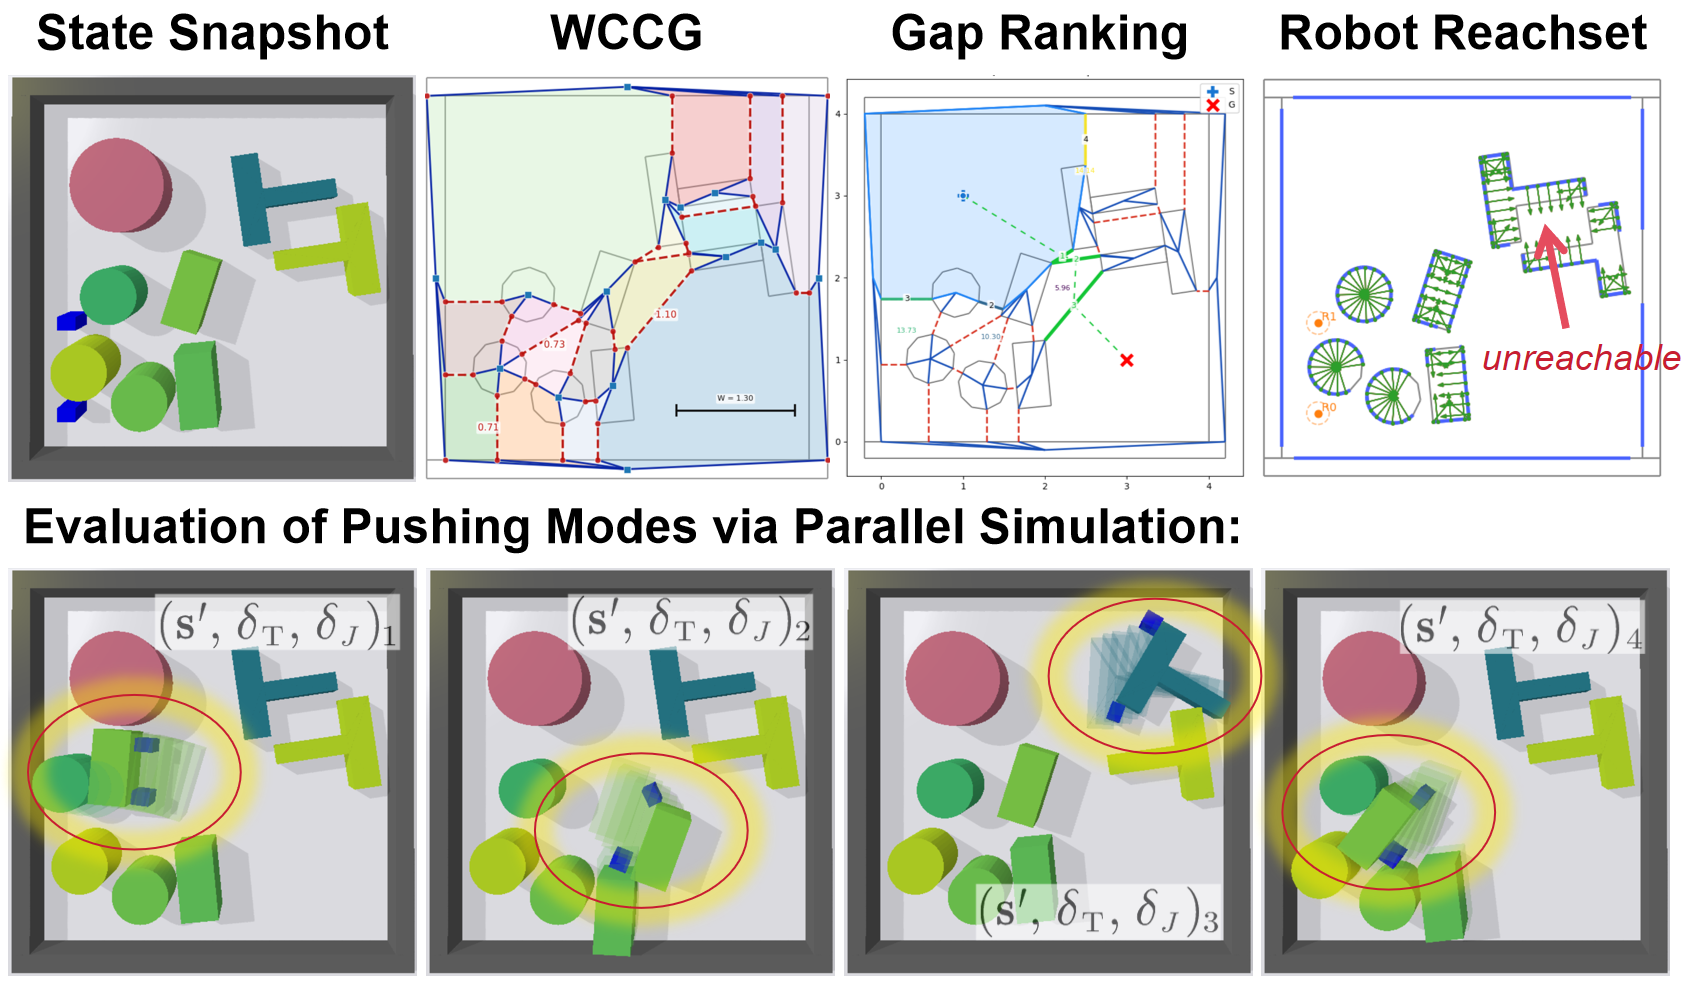
\includegraphics[width=0.95\linewidth]{figures/PIHS.png}
  \vspace{-0.15in}
  \caption{
  Overview of \textbf{PIHS} (physics–informed hybrid search). 
  \textbf{Top row (four panels):} (1) current simulation snapshot rendered in \texttt{PyBullet}; 
  (2) the corresponding $W$--clearance connectivity graph (WCCG); 
  (3) presearch on the WCCG with ranked candidate gaps (numbers indicate local/global ranks); 
  (4) robot \emph{reachable contacts} on obstacle boundaries (green arrows).
  \textbf{Bottom row:} given the current snapshot, the reachable contacts, and the ranked gaps, 
  PIHS samples push \emph{tasks} and \emph{modes} (e.g., face/edge, normal/tangential), 
  executes short-horizon physics rollouts, and visualizes the predicted outcomes: 
  ghosted trails show slider/object trajectories, and the final panel depicts the updated state used for the next search expansion.}
    \label{fig:PIHS}
   \vspace{-4mm}
\end{figure}
%------------------------------
\subsubsection{Node Selection}
At each iteration, the node with minimum best-first priority is selected from
the queue. The priority function balances the realized execution cost and the
estimated effort of remaining gaps:
\begin{equation}\label{eq:priority}
  f(\nu)\triangleq \chi(\nu)+\underset{g\in \textsf{Rank}(\nu)}{\textbf{min}}
  \widehat{\mathsf{Cost}}(g),
\end{equation}
where $\chi(\nu)$ is the cumulative execution cost so far, and the second term
is the minimum predicted remaining cost among the unexplored gaps of~$\nu$.
This scoring ensures that nodes are expanded in an order that jointly accounts
for physical effort already incurred and the most promising future actions.

\subsubsection{Node Expansion with Parallel Simulation}
When a node $\nu$ is selected for expansion, a batch of \emph{pushing
strategies} from $\mathsf{Rank}(\nu)$ is evaluated in parallel by simulation.
Each pushing strategy is defined as
\(\tau\triangleq(g,\mathbf{v},\boldsymbol{\xi})\), where
$g\in \boldsymbol{\Omega}$ is the chosen gap;
$\mathbf{v}\triangleq(v_x,v_y,\omega)\in \mathbb{R}^3$ is a short-horizon body
velocity for the manipulated obstacle;
and $\boldsymbol{\xi}\triangleq (\mathcal{C}_m,\mathbf{u}_m) \in (\partial\Omega_m)^N \times \mathbb{R}^{2N}$
is a contact mode specifying robot contact points and pushing forces as in~\eqref{eq:transition}.
Moreover, each candidate $\tau$ is first checked by a geometric quick-pass. If it passes,
it is evaluated by the simulator with the current state and pushing strategy:
\begin{equation}\label{eq:sim}
  (\mathbf{s}',\, \delta_\texttt{T},\, \delta_{\texttt{J}}) \triangleq \mathsf{EvalSim}
  \big{(}\nu,\, (g,\mathbf{v},\boldsymbol{\xi})\big{)},
\end{equation}
where $\mathbf{s}'$ is the successor state; $\delta_\texttt{T}>0$ is the time
cost; and $\delta_\texttt{J}$ is the control effort as in~\eqref{eq:problem}.
Thus, a successful evaluation produces a child
$\nu'\triangleq (\mathbf{s}',\pi')$, where $\pi'$ is obtained by appending
$\pi$ with $\tau$. The incremental realized cost of $\tau$ is
$\widehat{\mathsf{C}}(\nu,\,\tau)\triangleq \delta_\texttt{T} + \alpha\, \delta_\texttt{J}$,
with $\alpha>0$ the same trade-off parameter as in~\eqref{eq:problem}. The
cumulative cost is then updated by
$\chi(\nu')\triangleq \chi(\nu)+\widehat{\mathsf{C}}(\nu,\,\tau)$. Since many
pushing strategies are simulated concurrently, numerous successors can be
expanded in parallel at each iteration.

\subsubsection{Termination}
Termination occurs when a node $\nu$ reaches a state $\mathbf{s}$ for which a
$W$--clear path $\mathcal{P}^W_\texttt{V}$ exists from
$\mathbf{s}_\texttt{V}^{\texttt{S}}$ to $\mathbf{s}_\texttt{V}^{\texttt{G}}$,
as certified by~\eqref{eq:wccg_criterion}. In this case, the schedule $\pi$
stored in $\nu$ constitutes a complete solution to~\eqref{eq:problem}, encoding
both the sequence of gaps to clear and the physically feasible pushing actions
that realize them.

\begin{remark}[Parallel Expansion and Mode Reuse]\label{remark:simloop}
Efficiency of the hybrid search stems primarily from parallel evaluation of
pushing strategies, which allows many candidate futures to be simulated at once
for each expansion. Deferred expansion ensures that nodes with long candidate
lists remain in the priority queue until all tasks are attempted.
Moreover, validated $(\mathbf{v},\boldsymbol{\xi})$ pairs
are cached locally within a subtree and stored in a persistent ModeTable for
reuse across similar obstacles, significantly reducing repeated physics calls.
These mechanisms yield orders-of-magnitude speedup relative to naive
simulation-based search. \hfill$\blacksquare$
\end{remark}
